\documentclass[11pt,a4paper,twoside]{book}\usepackage[]{graphicx}\usepackage[]{xcolor}
% maxwidth is the original width if it is less than linewidth
% otherwise use linewidth (to make sure the graphics do not exceed the margin)
\makeatletter
\def\maxwidth{ %
  \ifdim\Gin@nat@width>\linewidth
    \linewidth
  \else
    \Gin@nat@width
  \fi
}
\makeatother

\definecolor{fgcolor}{rgb}{0.345, 0.345, 0.345}
\newcommand{\hlnum}[1]{\textcolor[rgb]{0.686,0.059,0.569}{#1}}%
\newcommand{\hlstr}[1]{\textcolor[rgb]{0.192,0.494,0.8}{#1}}%
\newcommand{\hlcom}[1]{\textcolor[rgb]{0.678,0.584,0.686}{\textit{#1}}}%
\newcommand{\hlopt}[1]{\textcolor[rgb]{0,0,0}{#1}}%
\newcommand{\hlstd}[1]{\textcolor[rgb]{0.345,0.345,0.345}{#1}}%
\newcommand{\hlkwa}[1]{\textcolor[rgb]{0.161,0.373,0.58}{\textbf{#1}}}%
\newcommand{\hlkwb}[1]{\textcolor[rgb]{0.69,0.353,0.396}{#1}}%
\newcommand{\hlkwc}[1]{\textcolor[rgb]{0.333,0.667,0.333}{#1}}%
\newcommand{\hlkwd}[1]{\textcolor[rgb]{0.737,0.353,0.396}{\textbf{#1}}}%
\let\hlipl\hlkwb

\usepackage{framed}
\makeatletter
\newenvironment{kframe}{%
 \def\at@end@of@kframe{}%
 \ifinner\ifhmode%
  \def\at@end@of@kframe{\end{minipage}}%
  \begin{minipage}{\columnwidth}%
 \fi\fi%
 \def\FrameCommand##1{\hskip\@totalleftmargin \hskip-\fboxsep
 \colorbox{shadecolor}{##1}\hskip-\fboxsep
     % There is no \\@totalrightmargin, so:
     \hskip-\linewidth \hskip-\@totalleftmargin \hskip\columnwidth}%
 \MakeFramed {\advance\hsize-\width
   \@totalleftmargin\z@ \linewidth\hsize
   \@setminipage}}%
 {\par\unskip\endMakeFramed%
 \at@end@of@kframe}
\makeatother

\definecolor{shadecolor}{rgb}{.97, .97, .97}
\definecolor{messagecolor}{rgb}{0, 0, 0}
\definecolor{warningcolor}{rgb}{1, 0, 1}
\definecolor{errorcolor}{rgb}{1, 0, 0}
\newenvironment{knitrout}{}{} % an empty environment to be redefined in TeX

\usepackage{alltt}
% We load package by package and set package relevant parameters.
% Topics are summarized later
%%%%%%%%%%%%%%%%%%%%%%%%%%%%%%%%%%%%%%%%%%%%%%%%%%%%%%%%%%%%%%%%%%%%%%%%
\usepackage{subcaption}
\usepackage{booktabs}
\usepackage{multicol}

% No-indent and increase spacing between paragraphs
\setlength\parindent{0pt}%Jerome
\setlength{\parskip}{0.2cm}
%%%%%%%%%%%%%%%%%%%%%%%%%%%%%%%%%%%%%%%%%%%%%%%%%%%%%%%%%%%%%%%%%%%%%%%%
% helping packages
\usepackage{ifthen}
\usepackage{calc}
\usepackage[T1]{fontenc}       % provides fonts having  accented characters 
\usepackage[latin1]{inputenc}  % allows the user to input accented characters directly from the keyboard

%%%%%%%%%%%%%%%%%%%%%%%%%%%%%%%%%%%%%%%%%%%%%%%%%%%%%%%%%%%%%%%%%%%%%%%%
\usepackage[latin1]{inputenc}
\usepackage{tikz}
\usetikzlibrary{shapes,arrows}
\usetikzlibrary{arrows.meta}
\usetikzlibrary{positioning,fit,calc}
\usepackage{varwidth}

%%%%%%%%%%%%%%%%%%%%%%%%%%%%%%%%%%%%%%%%%%%%%%%%%%%%%%%%%%%%%%%%%%%%%%%%

\renewcommand{\baselinestretch}{1.2}
\renewcommand{\textfraction}{0}%0.2     % placement of figures
\renewcommand{\topfraction}{1}%.3
\renewcommand{\bottomfraction}{1}%.3
\renewcommand{\floatpagefraction}{1}%.3
\setcounter{bottomnumber}{3}%1

\textwidth6.3in
\textheight9.7in
\topmargin-45pt
\oddsidemargin-.15in
\evensidemargin.15in
\headsep30pt
\headheight15pt
%\footskip20pt


%%%%%%%%%%%%%%%%%%%%%%%%%%%%%%%%%%%%%%%%%%%%%%%%%%%%%%%%%%%%%%%%%%%%%%%%

%\usepackage[dvipsnames]{xcolor} % 30.07.22 Commented out (Jerome)
\definecolor{fgcolor}{rgb}{0.345, 0.345, 0.345}
\definecolor{shadecolor}{rgb}{.97, .97, .97}
\definecolor{messagecolor}{rgb}{0, 0, 0}
\definecolor{warningcolor}{rgb}{1, 0, 1}
\definecolor{errorcolor}{rgb}{1, 0, 0}
\definecolor{DarkBlue}{rgb}{0,0,0.5451}
\definecolor{DarkGreen}{rgb}{0,0.39216,0}
\definecolor{LightYellow}{rgb}{1,1,.8}
\definecolor{orange}{rgb}{.9,0.3445,0}

\usepackage{soul}
\newcommand{\mathcolorbox}[2]{\colorbox{#1}{$\displaystyle #2$}}



%%%%%%%%%%%%%%%%%%%%%%%%%%%%%%%%%%%%%%%%%%%%%%%%%%%%%%%%%%%%%%%%%%%%%%%%
\usepackage{afterpage}
\usepackage{natbib}
\usepackage{upquote}

\usepackage[english]{babel}

% \newfloat{rcode}{h!t}{rcode}
% \floatname{rcode}{Code Example}

%%%%%%%%%%%%%%%%%%%%%%%%%%%%%%%%%%%%%%%%%%%%%%%%%%%%%%%%%%%%%%%%%%%%%%%%%%%%%%%
%% maxwidth is the original width if it is less than linewidth
%% otherwise use linewidth (to make sure the graphics do not exceed the margin)
\makeatletter
\def\maxwidth{ %
  \ifdim\Gin@nat@width>\linewidth
    \linewidth
  \else
    \Gin@nat@width
  \fi
}
\makeatother

%%%%%%%%%%%%%%%%%%%%%%%%%%%%%%%%%%%%%%%%%%%%%%%%%%%%%%%%%%%%%%%%%%%%%%%%%%%%%%%%%%%%%%%%%%%%%%%%%%%%%%%%%%%%
% from fancyvrb
\usepackage{fancyhdr}
\usepackage{fancyvrb}
\DefineVerbatimEnvironment{Rcode}{Verbatim}{xleftmargin=2em,fontshape=sl,formatcom=\color{DarkGreen}}
\fvset{listparameters={\setlength{\topsep}{0pt}}}

%%%%%%%%%%%%%%%%%%%%%%%%%%%%%%%%%%%%%%%%%%%%%%%%%%%%%%%%%%%%%%%%%%%%%%%%%%%%%%%%%%%%%%%%%%%%%%%%%%%%%%%%%%%%%
\usepackage{float}
\usepackage{graphicx}
\usepackage[margin=2em,labelfont=bf]{caption}

% Code float
\floatstyle{ruled}
\newfloat{program}{h!t}{ext}
\floatname{program}{\textsf{R}-Code}

%%%%%%%%%%%%%%%%%%%%%%%%%%%%%%%%%%%%%%%%%%%%%%%%%%%%%%%%%%%%%%%%%%%%%%%%
% allcolors = black makes the references black
\usepackage[pdftex,plainpages=false,pdfpagelabels,pagebackref=true,colorlinks=true,pdfpagemode=UseOutlines]{hyperref}


%%%%%%%%%%%%%%%%%%%%%%%%%%%%%%%%%%%%%%%%%%%%%%%%%%%%%%%%%%%%%%%%%%%%%%%%
% now math stuff and other details...
\usepackage{amsmath,amsthm,amssymb}
%\usepackage{amsfonts}
%\usepackage{bm}


\newtheorem{pro}{Property}[chapter]
\theoremstyle{definition}
\newtheorem{des}{Definition}[chapter]
\newtheorem{bsp}{Example}[chapter]
\newtheorem{rem}{Remark}[chapter]

\newcommand*\widebar[1]{%
  \vbox{%
    \hrule height 0.5pt%     % Line above with certain width
    \kern0.5ex%             % Distance between line and content
    \hbox{%
      \kern-0.1em%           % Distance between content and left side of box, negative values for lines shorter than content
      \ifmmode#1\else\ensuremath{#1}\fi%  % The content, typeset in dependence of mode
      \kern-0.1em%      % Distance between content and left side of box, negative values for lines shorter than content
    }% end of hbox
  }% end of vbox
}
\def\ds{\displaystyle}

\newcommand{\rr}[1]{{\ttfamily\slshape\color{DarkGreen} #1}}

\makeatletter


% clever trick to circumvent potential redefines after loading packages:
% \providecommand{\something}{}  % if it does not exist, it creates it.
%      has same syntax as \newcommand
% \renewcommand{\something}{....}
% TUGboat 29(2)


\makeatletter
%umdefinierung exisitierender befehle
\let\oldH\H
\let\oldL\L
\let\oldO\H
\let\oldS\S
\let\olda\a
\let\oldb\b
\let\oldc\c
\let\oldd\d
\let\oldk\k
\let\oldv\v
\let\oldl\l
\let\oldt\t
\let\oldu\u
\let\oldIJ\IJ
\let\oldP\P
\let\P\relax
\let\oldnorm\|

%\DefineVerbatimEnvironment{CodeInput}{Verbatim}{fontshape=sl}
%\DefineVerbatimEnvironment{CodeOutput}{Verbatim}{}

% some classical environments, up-right, with chapter numbering.
\theoremstyle{definition}
\newtheorem{definition}{Definition}[chapter]
\newtheorem{example}{Example}[chapter]
\newtheorem{remark}{Remark}[chapter]
\newtheorem{theorem}{Theorem}[chapter]



\renewcommand{\|}{|\!|}         % closer norm
\newcommand{\T}{{}^{\top}}
\newcommand\code[1]{{\tt#1}}



\newcounter{algo}
\newenvironment{algorithm}{%
  \begin{list}{
      (\arabic{algo})
    }{
      \usecounter{algo}
    }%
}{
  \end{list}
}

% some text abbreviation
\newcommand{\GLS}{\text{GLS}}
\newcommand{\RR}{\text{RR}}
\newcommand{\OR}{\text{OR}}
\newcommand{\WLS}{\text{WLS}}
\newcommand{\MLE}{\text{MLE}}
\newcommand{\OLS}{\text{OLS}}
\newcommand{\MAE}{\text{MAE}}
\newcommand{\MAD}{\text{MAD}}
\newcommand{\RMSE}{\text{RMSE}}

\newcommand{\ii}{\text{\i}}

\newcommand{\Bin}{\cB\mathit{\!i\!n}}
\newcommand{\Beta}{\cB\mathit{\!e\!t\!a}}
\newcommand{\Pois}{\cP\mathit{\!o\!i\!s\!s\!o\!n}}
\newcommand{\Exp}{\cE\mathit{\!x\!p}}


\DeclareMathOperator*{\argmin}{argmin}
\DeclareMathOperator*{\argmax}{argmax}
\DeclareMathOperator{\diag}{diag}
\DeclareMathOperator{\diam}{diam}
\DeclareMathOperator{\card}{card}
\DeclareMathOperator{\cov}{Cov}                   
\DeclareMathOperator{\corr}{Corr}                 
\DeclareMathOperator{\var}{Var}                   
\DeclareMathOperator{\trace}{tr}                  
\DeclareMathOperator{\E}{\mathbb{E}}%Jerome                  
\DeclareMathOperator{\P}{\mathbb{P}}%Jerome  
\DeclareMathOperator{\N}{\mathcal{N}}%Jerome                  
\DeclareMathOperator{\R}{\mathbb{R}}%Jerome 
\DeclareMathOperator{\se}{se}%Jerome             


\newcommand{\tram}{\text{tram}}%Jerome  
\newcommand{\mycomment}[1]{}
\newcommand{\abs}[1]{\ensuremath{\left\vert#1\right\vert}}%jerome


\DeclareMathOperator{\pred}{p}
\DeclareMathOperator{\vect}{vec}                  
\DeclareMathOperator{\vech}{vech}                 
\DeclareMathOperator{\rank}{rank}                 
\DeclareMathOperator{\e}{e}                       
%\DeclareMathOperator{\cv}{CV}                     
\DeclareMathOperator{\GCV}{GCV}                     
\DeclareMathOperator{\CV}{CV}                     
\DeclareMathOperator{\BLUP}{BLUP}                 
\DeclareMathOperator{\MSE}{MSE}                   
\DeclareMathOperator{\MS}{MS}                   
\DeclareMathOperator{\df}{df}                   
\DeclareMathOperator{\bias}{bias}                   
\DeclareMathOperator{\eig}{eig}                   
\DeclareMathOperator{\Prec}{Prec}
\DeclareMathOperator{\mode}{mode}
\renewcommand{\SS}{\text{SS}}
\renewcommand{\d}{\mathsf{\,d}}

\def\arctanh{\qopname\relax o{arctanh}}  % as in amsopn
\newcommand{\bigo}{\cO}
\newcommand{\lito}{\text{\scriptsize{$\cO$}}}
\newcommand{\cdfPhi}{\itPhi}
\newcommand{\ml}{_\text{ML}}

\newcommand*{\stack@relbin}[3][]{%
  \mathop{#3}\limits
  \toks@{#1}%
  \edef\reserved@a{\the\toks@}%
  \ifx\reserved@a\@empty\else_{#1}\fi
  \toks@{#2}%
  \edef\reserved@a{\the\toks@}%
  \ifx\reserved@a\@empty\else^{#2}\fi
  \egroup
}%
\renewcommand*{\stackrel}{\mathrel\bgroup\stack@relbin}
\newcommand*{\stackbin}{\mathbin\bgroup\stack@relbin}
\newcommand{\simiid}{\stackrel[]{\text{iid}}{\sim}}

% Kalligraphischer Schriftsatz
\newcommand{\cA}{{\cal{A}}}
\newcommand{\cB}{{\cal{B}}} 
\newcommand{\cC}{{\cal{C}}}
\newcommand{\cD}{{\cal{D}}} 
\newcommand{\cE}{{\cal{E}}}
\newcommand{\cF}{{\cal{F}}}
\newcommand{\cG}{{\cal{G}}}
\newcommand{\cH}{{\cal{H}}}
\newcommand{\cI}{{\cal{I}}}
\newcommand{\cJ}{{\cal{J}}}
\newcommand{\cK}{{\cal{K}}}
\newcommand{\cL}{{\cal{L}}}
\newcommand{\cM}{{\cal{M}}} 
\newcommand{\cN}{{\cal{N}}}
\newcommand{\cO}{{\cal{O}}} 
\newcommand{\cP}{{\cal{P}}}
\newcommand{\cQ}{{\cal{Q}}} 
\newcommand{\cR}{{\cal{R}}} 
\newcommand{\cS}{{\cal{S}}} 
\newcommand{\cT}{{\cal{T}}}
\newcommand{\cU}{{\cal{U}}}
\newcommand{\cV}{{\cal{V}}}
\newcommand{\cW}{{\cal{W}}}
\newcommand{\cX}{{\cal{X}}} 
\newcommand{\cY}{{\cal{Y}}}
\newcommand{\cZ}{{\cal{Z}}} 


\newcommand{\IA}{{\mathbb{A}}}
\newcommand{\IB}{{\mathbb{B}}}
\newcommand{\IC}{{\mathbb{C}}}
\newcommand{\ID}{{\mathbb{D}}}
\newcommand{\IE}{{\mathbb{E}}}
\newcommand{\IF}{{\mathbb{F}}}
\newcommand{\IG}{{\mathbb{G}}}
\newcommand{\IH}{{\mathbb{H}}}
\newcommand{\II}{{\mathbb{I}}}
%\newcommand{\IJ}{{\mathbb{J}}}
\newcommand{\IK}{{\mathbb{K}}}
\newcommand{\IL}{{\mathbb{L}}}
\newcommand{\IM}{{\mathbb{M}}}
\newcommand{\IN}{{\mathbb{N}}}
\newcommand{\IO}{{\mathbb{O}}}
\newcommand{\IP}{{\mathbb{P}}}
\newcommand{\IQ}{{\mathbb{Q}}}
\newcommand{\IR}{{\mathbb{R}}}
\newcommand{\IS}{{\mathbb{S}}}
\newcommand{\IT}{{\mathbb{T}}}
\newcommand{\IU}{{\mathbb{U}}}
\newcommand{\IV}{{\mathbb{V}}}
\newcommand{\IW}{{\mathbb{W}}}
\newcommand{\IX}{{\mathbb{X}}}
\newcommand{\IY}{{\mathbb{Y}}}
\newcommand{\IZ}{{\mathbb{Z}}}


% fette griechische kleinbuchstaben
\newcommand{\balpha}{{\boldsymbol{\alpha}}}
\newcommand{\bbeta}{{\boldsymbol{\beta}}}
\newcommand{\hbbeta}{{\boldsymbol{\hat\beta}}} % Jerome

\newcommand{\bgamma}{{\boldsymbol{\gamma}}}
\newcommand{\bdelta}{{\boldsymbol{\delta}}}
\newcommand{\blambda}{{\boldsymbol{\lambda}}}
\newcommand{\bepsilon}{{\boldsymbol{\epsilon}}}
\newcommand{\bvarepsilon}{{\boldsymbol{\varepsilon}}}
\newcommand{\bzeta}{{\boldsymbol{\zeta}}}
\newcommand{\bfeta}{{\boldsymbol{\eta}}}  %  <----- exception !
\newcommand{\btheta}{{\boldsymbol{\theta}}{}}
\newcommand{\bvartheta}{{\boldsymbol{\vartheta}}}
\newcommand{\biota}{{\boldsymbol{\iota}}}
\newcommand{\bkappa}{{\boldsymbol{\kappa}}}
\newcommand{\bmu}{{\boldsymbol{\mu}}}
\newcommand{\bnu}{{\boldsymbol{\nu}}}
\newcommand{\bxi}{{\boldsymbol{\xi}}}
\newcommand{\bpi}{{\boldsymbol{\pi}}}
\newcommand{\bvarpi}{{\boldsymbol{\varpi}}}
\newcommand{\brho}{{\boldsymbol{\rho}}}
\newcommand{\bvarrhoi}{{\boldsymbol{\varrho}}}
\newcommand{\bsigma}{{\boldsymbol{\sigma}}}
\newcommand{\bvarsigma}{{\boldsymbol{\varsigma}}}
\newcommand{\btau}{{\boldsymbol{\tau}}}
\newcommand{\bvartau}{{\boldsymbol{\vartau}}}
\newcommand{\bupsilon}{{\boldsymbol{\upsilon}}}
\newcommand{\bphi}{{\boldsymbol{\phi}}}
\newcommand{\bvarphi}{{\boldsymbol{\varphi}}}
\newcommand{\bchi}{{\boldsymbol{\chi}}}
\newcommand{\bpsi}{{\boldsymbol{\psi}}}
\newcommand{\bomega}{{\boldsymbol{\omega}}}


% fette griechische grossbuchstaben
\newcommand{\bGamma}{{\boldsymbol{\Gamma}}}
\newcommand{\bDelta}{{\boldsymbol{\Delta}}}
\newcommand{\bTheta}{{\boldsymbol{\Theta}}}
\newcommand{\bLambda}{{\boldsymbol{\Lambda}}{}}
\newcommand{\bXi}{{\boldsymbol{\Xi}}}
\newcommand{\bPi}{{\boldsymbol{\Pi}}}
\newcommand{\bSigma}{{\boldsymbol{\Sigma}}{}}
\newcommand{\bUpsilon}{{\boldsymbol{\Upsilon}}{}}
\newcommand{\bPhi}{{\boldsymbol{\Phi}}}
\newcommand{\bPsi}{{\boldsymbol{\Psi}}}
\newcommand{\bOmega}{{\boldsymbol{\Omega}}}
\newcommand{\bI}{{\boldsymbol{I}}}
\newcommand{\bV}{{\boldsymbol{V}}}
\newcommand{\bD}{{\boldsymbol{D}}}


% italics griechische grossbuchstaben
\newcommand{\itGamma}{{\mathit{\Gamma}}}
\newcommand{\itDelta}{{\mathit{\Delta}}}
\newcommand{\itTheta}{{\mathit{\Theta}}}
\newcommand{\itLambda}{{\mathit{\Lambda}}}
\newcommand{\itXi}{{\mathit{\Xi}}}
\newcommand{\itPi}{{\mathit{\Pi}}}
\newcommand{\itSigma}{{\mathit{\Sigma}}}
\newcommand{\itUpsilon}{{\mathit{\Upsilon}}}
\newcommand{\itPhi}{{\mathit{\Phi}}}
\newcommand{\itPsi}{{\mathit{\Psi}}}
\newcommand{\itOmega}{{\mathit{\Omega}}}



\newcommand{\A}{{\mathbf{A}}}
\newcommand{\B}{{\mathbf{B}}}
\newcommand{\C}{{\mathbf{C}}}
\newcommand{\D}{{\mathbf{D}}}
\newcommand{\bfE}{{\mathbf{E}}}    % \E: expectation
\newcommand{\F}{{\mathbf{F}}}
\newcommand{\G}{{\mathbf{G}}}
\renewcommand{\H}{{\mathbf{H}}}
\newcommand{\I}{{\mathbf{I}}}
\newcommand{\J}{{\mathbf{J}}}
\newcommand{\K}{{\mathbf{K}}}
\renewcommand{\L}{{\mathbf{L}}}
\newcommand{\bfM}{{\mathbf{M}}}
%\newcommand{\N}{{\mathbf{N}}}%Jerome
\renewcommand{\O}{{\mathbf{O}}}
\newcommand{\bfP}{{\mathbf{P}}}  % \P : probability
\newcommand{\Q}{{\mathbf{Q}}}
\newcommand{\bfR}{{\mathbf{R}}}
\renewcommand{\S}{{\mathbf{S}}}
\newcommand{\bfT}{{\mathbf{T}}} % \T transpose
\newcommand{\U}{{\mathbf{U}}}
\newcommand{\V}{{\mathbf{V}}}
\newcommand{\W}{{\boldsymbol{W}}}
\newcommand{\X}{{\boldsymbol{X}}}% IMPORTANT**************************************************
\newcommand{\bR}{{\boldsymbol{R}}}
\newcommand{\M}{{\boldsymbol{M}}}
\newcommand{\Y}{{\mathbf{Y}}}
\newcommand{\Z}{{\mathbf{Z}}}
\newcommand{\bE}{{\boldsymbol{E}}}
\newcommand{\be}{{\boldsymbol{e}}} %% Jerome
\newcommand{\bP}{{\boldsymbol{P}}} %% Jerome


\newcommand{\0}{{\mathbf{0}}}
\newcommand{\1}{{\mathbf{1}}}
\newcommand{\2}{{\mathbf{2}}}
\newcommand{\3}{{\mathbf{3}}}
\newcommand{\4}{{\mathbf{4}}}
\newcommand{\5}{{\mathbf{5}}}
\newcommand{\6}{{\mathbf{6}}}
\newcommand{\7}{{\mathbf{7}}}
\newcommand{\8}{{\mathbf{8}}}
\newcommand{\9}{{\mathbf{9}}}

\renewcommand{\a}{{\textbf{\textit{a}}}}
\renewcommand{\b}{{\textbf{\textit{b}}}}
\renewcommand{\c}{{\textbf{\textit{c}}}}
\newcommand{\bfd}{{\textbf{\textit{d}}}}  % \d  'dx'
\newcommand{\bfe}{{\textbf{\textit{e}}}}  % \e  l'exponentiel
\newcommand{\f}{{\textbf{\textit{f}}}}
\newcommand{\g}{{\textbf{\textit{g}}}}
\newcommand{\h}{{\textbf{\textit{h}}}}
\newcommand{\bfi}{{\textbf{\textit{i}}}}%\i  complex i, sans 'dot'
\newcommand{\bfj}{{\textbf{\textit{j}}}}
\renewcommand{\l}{{\textbf{\textit{l}}}}
\renewcommand{\k}{{\textbf{\textit{k}}}}
\newcommand{\m}{{\textbf{\textit{m}}}}
\newcommand{\bfn}{{\textbf{\textit{n}}}}
\newcommand{\bfo}{{\textbf{\textit{o}}}}
\newcommand{\p}{{\textbf{\textit{p}}}}
\newcommand{\q}{{\textbf{\textit{q}}}}
\renewcommand{\r}{{\textbf{\textit{r}}}}
\newcommand{\s}{{\textbf{\textit{s}}}}
\renewcommand{\t}{{\textbf{\textit{t}}}}
\newcommand{\bfu}{{\textbf{\textit{u}}}} %\u used in references
\renewcommand{\v}{{\textbf{\textit{v}}}}
\newcommand{\w}{{\textbf{\textit{w}}}}
\newcommand{\x}{{\textbf{\textit{x}}}}
\newcommand{\y}{{\textbf{\textit{y}}}}
\newcommand{\z}{{\textbf{\textit{z}}}}



\newcommand{\hb}{{\boldsymbol{\hat{{b}}}}} %Jerome
\newcommand{\hy}{{\boldsymbol{\hat{y}}}} % Jerome
\newcommand{\hbt}{{\boldsymbol{\hat{t}}}} % Jerome
\newcommand{\hX}{{\boldsymbol{\hat{X}}}} % Jerome



\ifcsname hlkwd\endcsname%    ... command '#1' exists ...%
\else%  ... command '#1' does not exist ...%

\def\maxwidth{ %
  \ifdim\Gin@nat@width>\linewidth
    \linewidth
  \else
    \Gin@nat@width
  \fi
}

\definecolor{fgcolor}{rgb}{0.345, 0.345, 0.345}
\newcommand{\hlnum}[1]{\textcolor[rgb]{0.686,0.059,0.569}{#1}}%
\newcommand{\hlstr}[1]{\textcolor[rgb]{0.192,0.494,0.8}{#1}}%
\newcommand{\hlcom}[1]{\textcolor[rgb]{0.678,0.584,0.686}{\textit{#1}}}%
\newcommand{\hlopt}[1]{\textcolor[rgb]{0,0,0}{#1}}%
\newcommand{\hlstd}[1]{\textcolor[rgb]{0.345,0.345,0.345}{#1}}%
\newcommand{\hlkwa}[1]{\textcolor[rgb]{0.161,0.373,0.58}{\textbf{#1}}}%
\newcommand{\hlkwb}[1]{\textcolor[rgb]{0.69,0.353,0.396}{#1}}%
\newcommand{\hlkwc}[1]{\textcolor[rgb]{0.333,0.667,0.333}{#1}}%
\newcommand{\hlkwd}[1]{\textcolor[rgb]{0.737,0.353,0.396}{\textbf{#1}}}%

\usepackage{framed}
\newenvironment{kframe}{%
 \def\at@end@of@kframe{}%
 \ifinner\ifhmode%
  \def\at@end@of@kframe{\end{minipage}}%
  \begin{minipage}{\columnwidth}%
 \fi\fi%
 \def\FrameCommand##1{\hskip\@totalleftmargin \hskip-\fboxsep
 \colorbox{shadecolor}{##1}\hskip-\fboxsep
     % There is no \\@totalrightmargin, so:
     \hskip-\linewidth \hskip-\@totalleftmargin \hskip\columnwidth}%
 \MakeFramed {\advance\hsize-\width
   \@totalleftmargin\z@ \linewidth\hsize
   \@setminipage}}%
 {\par\unskip\endMakeFramed%
 \at@end@of@kframe}
\renewenvironment{kframe}{%
 \def\at@end@of@kframe{}%
 \ifinner\ifhmode%
  \def\at@end@of@kframe{\end{minipage}}%
  \begin{minipage}{\columnwidth}%
 \fi\fi%
 \def\FrameCommand##1{\hskip\@totalleftmargin \hskip-0\fboxsep
 \colorbox{shadecolor}{##1}\hskip-0\fboxsep
     % There is no \\@totalrightmargin, so:
     \hskip-\linewidth \hskip-\@totalleftmargin \hskip\columnwidth}%
 \MakeFramed {\advance\hsize-\width
   \@totalleftmargin\z@ \linewidth\hsize
   \@setminipage}}%
 {\par\unskip\endMakeFramed%
 \at@end@of@kframe}


\definecolor{shadecolor}{rgb}{.97, .97, .97}
\definecolor{messagecolor}{rgb}{0, 0, 0}
\definecolor{warningcolor}{rgb}{1, 0, 1}
\definecolor{errorcolor}{rgb}{1, 0, 0}
%\newenvironment{knitrout}{}{} % an empty environment to be redefined in TeX
\newenvironment{knitrout}{\setlength{\topsep}{0mm}\setlength{\fboxsep}{4mm}}{} 

\usepackage{alltt}
\IfFileExists{upquote.sty}{\usepackage{upquote}}{}

  \fi%

\makeatother
   % packages, layout and standard macros
\IfFileExists{upquote.sty}{\usepackage{upquote}}{}
\begin{document}
\renewcommand\familydefault{\sfdefault} 
\pagenumbering{Alph}


\thispagestyle{empty}
\renewcommand{\baselinestretch}{1.5}\normalfont
\begin{center}
\setlength{\parindent}{0cm}
\bf\Large% 
Assessment of the detrimental effects \\
of collinearity in \\
classical and transformation models
\normalfont

\hrulefill

\vspace*{4cm}

\large
Master Thesis in Biostatistics (STA495) % or choose the next one
% Master Thesis in Mathematics (MAT491) 
\vspace*{12mm}

by

\vspace*{12mm}

Jerome Sepin\\
\small 17-932-427\\
\normalfont
\vspace*{4cm}

supervised by

\vspace*{1cm}

PD Dr. Malgorzata Roos

\vfill

Zurich, \today
\end{center}
\renewcommand\familydefault{\rmdefault}%
\renewcommand{\baselinestretch}{1.0}\rm 
\setcounter{page}{0}
\newpage
\vspace*{12cm}~\thispagestyle{empty}\pagenumbering{Roman}
\newpage





\graphicspath{{./figure/}}
\DeclareGraphicsExtensions{.pdf,.png}
\setcounter{tocdepth}{2}

\thispagestyle{empty}
\begin{center}
  \vspace*{6cm}{\bfseries\Huge
  Assessment of the detrimental effects\\[5mm] of collinearity in \\[5mm] classical and transformation models
  }
  \vfill
  \rm

  \LARGE
  Jerome Sepin\\[12mm]
  
  \normalsize
  Version \today
\end{center}
\newpage
\thispagestyle{empty}~
\newpage
\pagenumbering{roman}

\chapter*{Acknowledgement}
I would like to express my sincere gratitude to everyone who has supported me during the completion of this thesis.
I am particularly grateful to my supervisor, PD Dr. Malgorzata Roos, for her guidance, insightful feedbacks, and unwavering support throughout the research process.
Without your help and infectious positive mindset, this would have never been possible.
Moreover, I would like to thank the whole teaching staff of the Biostatistics Master Program for doing their best in teaching statistics and making my time as student, both instructive and inspiring.

\bigskip
\begin{flushright}
  Jerome Sepin\\
  February 2023
\end{flushright}


\thispagestyle{plain}\markboth{Contents}{Contents}
\tableofcontents
\setkeys{Gin}{width=.8\textwidth}

\chapter*{Abstract}
\addtocontents{toc}{\protect \vspace*{13.mm}}
\addcontentsline{toc}{chapter}{\bfseries{Abstract}}
\thispagestyle{plain}\markboth{Abstract}{Abstract}

Multiple linear regression techniques are well-established statistical tools that are able to quantify the association between many explanatory variables and one outcome variable in a human-interpretable manner.
However, many explanatory variables increase the chance of collinearity, which means that one of them is well explainable by linear combinations of others.
It is well known that collinearity has detrimental impacts on multiple linear regression estimands, thus stimulating research on collinearity.
For example, Belsley came up with a rule of thumb to detect harmful collinearity, which says that condition indices, and therefore also condition numbers, over 30 indicate consequential collinearity.
In the meantime, this rule of thumb has been widely advocated so that it seems to be carved in stone.
Therefore, it is important to design a Monte Carlo simulation to clarify the relevance of this cut-off.

Belsley's rule of thumb applies to the omnipresent statistical workhorse, the least-squares model.
However, with the rise of computational power, novel transformation models that are able to flexibly transform the outcome have a large impact on the understanding of regression models.
It is currently not known whether both, least-squares and the transformation model equivalent, react equally to collinearity.
Thus, it is important to clarify whether collinearity diagnostics procedure developed with least-squares can also be used in transformation models.

Furthermore, it can be expected that the sample size can mitigate the detrimental impact of collinearity, but there are currently no exact rules how to do this.
Thus, there is a demand for software and well-explained hands-on examples that assist in properly adjusting the study design to account for collinearity.

To address these needs in this master thesis, we designed and conducted a Monte Carlo simulation study where we found no signs of tipping point at Belsley's cut-off value of 30.
However, we discovered that the degree of collinearity summarized by one condition number impacts the Wald statistics values of both, the least-squares model and the transformation model equivalent.
We also demonstrated that the Wald statistic values differ in general between the two methods.
Moreover, we proposed a method for sample size calculation in the least-squares case.
The methods developed are implemented in open-source \textsf{R} software, which is integrated in the \texttt{Collinearity} package.
As additional support, we also demonstrated how to apply these methods in a case study using the \texttt{BostonHousing2} data.
These examples and functions assess the impact of the detrimental effect of collinearity on multiple linear regression estimands and suggest how to improve the sample size to mitigate this detrimental effect.

% \bigskip
% \begin{flushright}
%   Jerome Sepin\\
%   February 2023
% \end{flushright}

\addtocontents{toc}{\protect \vspace*{10mm}}

\cleardoublepage
\pagenumbering{arabic}


%%%%%%%%%%%%%%%%%%%%%%%%%%%%%%%%%%%%%%%%%%%%%%%%%%%%%%%%%%%%%%%%%%%%%%


% LaTeX file for Chapter 01


%%%%%%%%%%%%%%%%%%%%%%%%%%%%%%%%%%%%%%%%%%%%%%%%%%%%%%%%%%%%%%%%%%%%%%%%%%%%%%%%
\chapter{Introduction}
%%%%%%%%%%%%%%%%%%%%%%%%%%%%%%%%%%%%%%%%%%%%%%%%%%%%%%%%%%%%%%%%%%%%%%%%%%%%%%%%

Multiple linear regression techniques are well-established and easy-interpretable statistical tools that can incorporate many explanatory variables associated with one outcome variable. Many explanatory variables increase the chance of collinearity, which means that one of them is well explained by a linear combination of others. It is well known that collinearity has detrimental impacts on multiple linear regression estimands.


%%%%%%%%%%%%%%%%%%%%%%%%%%%%%%%%%%%%%%%%%%%%%%%%%%%%%%%%%%%%%%%%%%%%%%


% LaTeX file for Chapter 02


\chapter{Causal inference from complex longitudinal data}\label{chap:methods}

This chapter summarizes \cite{hernan2023} part III.

%%%%%%%%%%%%%%%%%%%%%%%%%%%%%%%%%%%%%%%%%%%%%%%%%%
\section{TIME-VARYING TREATMENTS (19)}
%%%%%%%%%%%%%%%%%%%%%%%%%%%%%%%%%%%%%%%%%%%%%%%%%%

% %%%%%%%%%%%%%%%%
\subsection{The causal effect of time-varying treatments (19.1)}
% %%%%%%%%%%%%%%%%


time-varying dichotomous treatment $A_k$ at time $k=0,1,2,\dots,K$

We refer to the treatment history as $\bar{A}_k=\left(A_0,\dots, A_K\right)$
Patients under treatment throughout the whole time $K$ have $\bar{A}=\left(A_0=1,\dots, A_K=1\right)=\bar{1}$ while patients that never receive treatment do have history $\bar{A}=\left(A_0=0,\dots, A_K=0\right)=\bar{0}$.
Most likely patients will have some sort of a mixture between those two treatment strategies due to various reasons and therefore a compact (and true) notation is not really possible.
The average treatment effect at timepoint $k$ may be defined as:

$$\E\left[Y^{a_k=1}\right]-\E\left[Y^{a_k=0}\right]$$

however, this does not reflect the overall goal to quantify the average causal effect of the time-varying treatment.
Due to the fact that in reality the treatment strategies cannot be completely discriminated between $\bar{1}$ or $\bar{0}$, no \textbf{unique} average causal effect is defined.

% %%%%%%%%%%%%%%%%
\subsection{Treatment strategies (19.2)}
% %%%%%%%%%%%%%%%%

"Always treat" vs. "Never treat": $\E\left[Y^{\bar{a}=\bar{1}}\right]-\E\left[Y^{\bar{a}=\bar{0}}\right]$

Dynamic treatment strategy: $a_k$ depends on the evolution of the patients time-varying covariate(s) $\bar{L}_k$ (otherwise they are called static). Development of ADA and subsequent discontinuation of the treatment is a form of dynamic treatment strategy.


The average causal effect estimate of a (potentially) time-varying treatment is only well defined if the strategies are specified (and hold). Since at each timepoint $k$ there is the option (random or deterministic) to treat or not to treat, there are a many different treatment strategies available resulting in \textbf{many} different causal effects. 

% %%%%%%%%%%%%%%%%
\subsection{Sequentially randomized experiments (19.3)}
% %%%%%%%%%%%%%%%%

%\newpage
\tikzstyle{block} = [draw=black, thick, text width=2cm, minimum height=1cm, align=center]
\tikzstyle{cloud} = [draw=black, ellipse, text width=1cm, minimum height=1cm, align=center] 
% \tikzstyle{cloud} = [draw, ellipse,fill=red!20, node distance=3cm,
%     minimum height=2em]
\tikzstyle{arrow} = [thick,->,>=stealth]

\begin{figure}[H]
\centering
\begin{tikzpicture}

    \node[cloud] (L0) {$L_0$};
    \node[cloud, right=of L0, xshift=-0.2cm] (A0) {$A_0$};
    \node[cloud, right=of A0, xshift=0.9cm] (L1) {$L_1$};
    \node[cloud, right=of L1, xshift=-0.2cm] (A1) {$A_1$};
    
    % outcome
    \node[cloud, right=of A1, xshift=0.9cm] (Y) {$Y$};
    
    % unobserved confounders
    \node[cloud, below=of L0, yshift=-0.7cm] (U0) {$U_0$};
    \node[cloud, below=of L1, yshift=-0.7cm] (U1) {$U_1$};
    
    % edges
    \draw [arrow] (L0) -- (A0);
    \draw [arrow] (L0) to [out=45,in=135]  (L1);
    \draw [arrow] (L0) to [out=45,in=135]  (A1);
    \draw [arrow] (L0) to [out=45,in=135]  (Y);
    
    
    \draw [arrow] (A0) -- (L1);
    \draw [arrow] (A0) -- (U1);
    \draw [arrow] (A0) to [out=45,in=150]  (A1);
    \draw [arrow] (A0) to [out=45,in=150]  (Y);
    
    
    \draw [arrow] (L1) -- (A1);
    \draw [arrow] (L1) to [out=45,in=160]  (Y);
    
    \draw [arrow] (A1) -- (Y);
    
    \draw [arrow] (U0) -- (L0);
    \draw [arrow] (U0) -- (L1);
    \draw [arrow] (U0) -- (U1);
    \draw [arrow] (U0) to [out=-45,in=-90]  (Y);
    
    \draw [arrow] (U1) -- (L1);
    \draw [arrow] (U1) -- (Y);

    
\end{tikzpicture}
\caption{Causal diagram of a randomized clinical trial with dynamic treatment strategy, meaning that depending on some of the patients covariates, the treatment may be changed. Corresponds to Figure 19.2 in \cite{hernan2023}}\label{fig:19.1}
\end{figure}

% %%%%%%%%%%%%%%%%
\subsection{Sequential exchangeability (19.4)}
% %%%%%%%%%%%%%%%%

Causal inference (unbiased effect estimation) with time-fixed treatment effects require conditional exchangeability $Y^a \perp A\mid L$ 

(\textcolor{red}{p247: "Conditional exchangeability holds in observational studies if the probability of receiving treatment depends on the measured covariates L and, conditional on L, does not further depend on any unmeasured, common causes of treatment and outcome."})

Sequential conditional exchangeability:
\begin{align}
Y^g \perp A_k\mid \bar{A}_{k-1}=g\left(\bar{A}_{k-2}, \bar{L}_{k-1}\right),\bar{L}_k\label{eq:seqexch}
\end{align}

% %%%%%%%%%%%%%%%%
\subsection{Identifiability under some but not all treatment strategies (19.5)}
% %%%%%%%%%%%%%%%%

\textcolor{red}{Needs knowledge of $d$-separation and SWIG.}


% %%%%%%%%%%%%%%%%
\subsection{Time-varying confounding and time-varying confounders (19.6)}
% %%%%%%%%%%%%%%%%

p253: "\textit{Achieving approximate exchangeability requires expert knowledge,
which will guide investigators in the design of their studies to measure as
many of the relevant variables $\bar{L}_k$ as possible. For example, in an HIV study, experts would agree that time-varying variables like CD4 cell count, viral load, symptoms need to be appropriately measured and adjusted for.}"

p253: "\textit{But the question "Are the measured covariates sufficient to ensure sequential exchangeability?" can never be answered with certainty.}"

%%%%%%%%%%%%%%%%%%%%%%%%%%%%%%%%%%%%%%%%%%%%%%%%%%
\section{TREATMENT-CONFOUNDER FEEDBACK (20)}
%%%%%%%%%%%%%%%%%%%%%%%%%%%%%%%%%%%%%%%%%%%%%%%%%%

"\textit{Suppose that we have a study in which the strongest form of sequential exchangeability holds:
the measured time-varying confounders are sufficient to validly estimate the causal effect of any treatment strategy.
Then the question is what confounding adjustment method to use.
The answer to this question highlights a key problem in causal inference about time-varying treatments: treatment-confounder feedback.}"

If treatment-confounder feedback is apparent, traditional adjustment methods induce bias.

% %%%%%%%%%%%%%%%%
\subsection{The elements of treatment-confounder feedback (20.1)}
% %%%%%%%%%%%%%%%%



\begin{figure}[H]
\centering
\begin{tikzpicture}

    \node[cloud] (L0) {$L_0$};
    \node[cloud, right=of L0, xshift=-0.2cm] (A0) {$A_0$};
    \node[cloud, right=of A0, xshift=0.9cm] (L1) {$L_1$};
    \node[cloud, right=of L1, xshift=-0.2cm] (A1) {$A_1$};
    
    % outcome
    \node[cloud, right=of A1, xshift=0.9cm] (Y) {$Y$};
    
    % unobserved confounders
    \node[cloud, below=of L0, yshift=-0.7cm] (U0) {$U_0$};
    \node[cloud, below=of L1, yshift=-0.7cm] (U1) {$U_1$};
    
    % edges
    \draw [arrow] (L0) -- (A0);
    \draw [arrow] (L0) to [out=45,in=135]  (L1);
    \draw [arrow] (L0) to [out=45,in=135]  (A1);
    \draw [arrow] (L0) to [out=45,in=135]  (Y);
    
    
    \draw [arrow, red] (A0) -- (L1);
    \draw [arrow, red] (A0) -- (U1);
    \draw [arrow] (A0) to [out=45,in=150]  (A1);
    \draw [arrow] (A0) to [out=45,in=150]  (Y);
    
    
    \draw [arrow] (L1) -- (A1);
    \draw [arrow] (L1) to [out=45,in=160]  (Y);
    
    \draw [arrow] (A1) -- (Y);
    
    \draw [arrow] (U0) -- (L0);
    \draw [arrow] (U0) -- (L1);
    \draw [arrow] (U0) -- (U1);
    \draw [arrow] (U0) to [out=-45,in=-90]  (Y);
    
    \draw [arrow] (U1) -- (L1);
    \draw [arrow] (U1) -- (Y);

    
\end{tikzpicture}
\caption{Corresponds to Figure 19.2 or 20.1 in \cite{hernan2023}. 
The \textbf{treatment-confounder feedback} means in this example that the confounder ($L_k$) affects the treatment ($A_k$) \texttt{and} the treatment ($A_k$) affects in-turn again the confounder ($L_{k+1}$). And this \textbf{treatment-confounder feedback} can be caused directly or even go over unmeasured variables $U_k$.
Remark: When the two red edges would be removed, we would still have time-varying confounders but not anymore treatment-confounder feedback.
}\label{fig:20.1}
\end{figure}

% % %%%%%%%%%%%%%%
\subsubsection{An example why traditional methods fail}
% % %%%%%%%%%%%%%%

\begin{figure}[H]
\centering
\begin{tikzpicture}

    \node[cloud] (L1) {$L_1$};
    \node[cloud, right=of L1, xshift=-0.2cm] (A1) {$A_1$};
    \node[cloud, left=of L1, xshift=-0.9cm] (A0) {$A_0$};
    % outcome
    \node[cloud, right=of A1, xshift=0.9cm] (Y) {$Y$};
    
    % unobserved confounders
    \node[cloud, below=of L1, yshift=-0.7cm] (U1) {$U_1$};
    
    % edges
    \draw [arrow] (A0) -- (L1);

    \draw [arrow] (L1) -- (A1);

    \draw [arrow] (U1) -- (L1);
    \draw [arrow] (U1) -- (Y);

    
\end{tikzpicture}
\caption{Corresponds to Figure 20.3 in \cite{hernan2023}. 
Illustrates a sequentially randomized trial with two time-points $k=0,1$. Furthermore, treatment $A_0$ is unconditionally (or marginally) randomized and $A_1$ is randomized only with respect to confounders $L_1$. 
Since no edge from $A_1, L_1, A_1$ to $Y$ is drawn, there is no effect assumed.
}\label{fig:20.3}
\end{figure}

We are interested in estimating the \textbf{average causal treatment effect} of the static treatment strategy "always treat" ($a_0=1,a_1=1$) versus the static treatment strategy "never treat" ($a_0=0,a_1=0$) on the outcome $Y$. Thus the \textbf{average causal treatment effect} is 
\begin{align}
\E\left[Y^{a_0=1,a_1=1}\right]-\E\left[Y^{a_0=0,a_1=0}\right] \label{eq:20.3}
\end{align}
and should be 0 since there are no forward directed paths possible from $A_0$ or $A_1$ to $Y$. In addition, since there are no edges from unmeasured variables $U$ into the treatment $A$, we can argue Figure~\ref{fig:20.3} represents indeed a randomized trial and thus we should be able to use originating data ($A_0, L_1, A_1, Y$) to conclude \eqref{eq:20.3} is equals to 0.


Even though if sequential exchangeability is given (when conditioning on confounder $L_1$), if we have time-varying confounders \textbf{and} treatment-confounder feedback, traditional methods can not correctly adjust for those confounder and thereby induce bias.


% %%%%%%%%%%%%%%%%
\subsection{The bias of traditional methods (20.2)}
% %%%%%%%%%%%%%%%%

\begin{table}[H]
\caption{Table 20.1 in \cite{hernan2023}}
\centering
% latex table generated in R 4.2.2 by xtable 1.8-4 package
% Tue Mar 21 15:31:22 2023
\begingroup\footnotesize
\begin{tabular}{rrrrr}
  \toprule
$A_0$ & $L_1$ & $A_1$ & $N$ & Mean $Y$ \\ 
  \midrule
0 & 0 & 0 & 2400 & 84 \\ 
  0 & 0 & 1 & 1600 & 84 \\ 
  0 & 1 & 0 & 2400 & 52 \\ 
  0 & 1 & 1 & 9600 & 52 \\ 
  1 & 0 & 0 & 4800 & 76 \\ 
  1 & 0 & 1 & 3200 & 76 \\ 
  1 & 1 & 0 & 1600 & 44 \\ 
  1 & 1 & 1 & 6400 & 44 \\ 
   \bottomrule
\end{tabular}
\endgroup

\end{table}
\begin{itemize}
\item $\P\left(A_0=1\right)=0.5$
\item $\P\left(A_1=1\mid L_1=0\right)=0.4$ and $\P\left(A_1=1\mid L_1=1\right)=0.8$
\end{itemize}


We can confirm the causal effects of $A_0$ and $A_1$ (conditinal on the past) are indeed zero when we treat $A_0$ and $A_1$ seperately as time-fixed treatments:
\begin{enumerate}
\item The average causal effect in the stratum $(A_0=0,L_1=0)$:
\begin{align*}
\E\left[Y^{a_1=1}\mid A_0=0,L_1=0\right]-\E\left[Y^{a_1=0}\mid A_0=0,L_1=0\right]=84-84=0
\end{align*}
\item The average causal effect in the stratum $(A_0=0,L_1=1)$:
\begin{align*}
\E\left[Y^{a_1=1}\mid A_0=0,L_1=1\right]-\E\left[Y^{a_1=0}\mid A_0=0,L_1=1\right]=52-52=0
\end{align*}
\item The average causal effect in the stratum $(A_0=1,L_1=0)$:
\begin{align*}
\E\left[Y^{a_1=1}\mid A_0=1,L_1=0\right]-\E\left[Y^{a_1=0}\mid A_0=1,L_1=0\right]=76-76=0
\end{align*}
\item The average causal effect in the stratum $(A_0=1,L_1=1)$:
\begin{align*}
\E\left[Y^{a_1=1}\mid A_0=1,L_1=1\right]-\E\left[Y^{a_1=0}\mid A_0=1,L_1=1\right]=44-44=0
\end{align*}
\end{enumerate}

Joining $A_0$ and $A_1$ as a joint time-varying treatment is not so easy even though the identifiablity conditions (\textcolor{red}{???}) hold and thus the data should be well enough to estimate the effect.
Comparing the two treatment strategies "always treat" versus "never treat":
\begin{align*}
\E\left[Y^{a_0=1,a_1=1}\right]-\E\left[Y^{a_0=0,a_1=0}\right]
\end{align*}
should be equals zero according to the $g$-null theorem (\textcolor{red}{???}).



With the classical methods this is however not the case:
\begin{align*}
\E\left[Y\mid A_0=1, A_1=1\right]-\E\left[Y\mid A_0=0, A_1=0\right]&=54.6666667-68=-13.3333333\\
\E\left[Y\mid A_0=1,L_1=0, A_1=1\right]-\E\left[Y\mid A_0=0,L_1=0,A_1=0\right]&=76-84=-8\\
\E\left[Y\mid A_0=1,L_1=1, A_1=1\right]-\E\left[Y\mid A_0=0,L_1=0,A_1=0\right]&=44-52=-8
\end{align*}


% %%%%%%%%%%%%%%%%
\subsection{Why traditional methods fail (20.3)}
% %%%%%%%%%%%%%%%%

Stratification can not handle treatment-confounder feedback

In our example in Figure~\ref{fig:20.3}, stratification with respect to $L_1$ is problematic. This, because $L_1$ is a collider for association measure $A_0$ and thus opens the path $A_0\rightarrow L_1 \leftarrow U_1\rightarrow Y$.
This means that stratification induces a non-causal relationship between treatment $A_0$ and unmeasured variable $U_1$ and therefore also between $A_0$ and outcome $Y$, within levels of $L_1$.
Thereby, stratification for $L_1$ eliminates confounding for $A_1$ but introduces \textbf{selection bias} for $A_0$.


%%%%%%%%%%%%%%%%%%%%%%%%%%%%%%%%%%%%%%%%%%%%%%%%%%
\section{G-METHODS FOR TIME-VARYING TREATMENTS (21)}
%%%%%%%%%%%%%%%%%%%%%%%%%%%%%%%%%%%%%%%%%%%%%%%%%%


% %%%%%%%%%%%%%%%%
\subsection{The g-formula for time-varying treatments (21.1)}
% %%%%%%%%%%%%%%%%




%%%%%%%%%%%%%%%%%%%%%%%%%%%%%%%%%%%%%%%%%%%%%%%%%%
\newpage
\section{Transformation models}\label{sec:trans_model}
%%%%%%%%%%%%%%%%%%%%%%%%%%%%%%%%%%%%%%%%%%%%%%%%%%

\cite{Hothorn2020} nicely proposes a prospective to unify a wide range of statistical models by moving to conditional distributions and thus leaves the models relying on conditional expectation behind. We get there by rearranging the familiar model, noted by Equation, to model the error term $\bvarepsilon$ as
\begin{align*}
\frac{\y-\boldsymbol{X\beta}}{\sigma}&=\boldsymbol{\varepsilon}
\end{align*}
This is done because the error term $\bvarepsilon$ is the only stochastic component of the model and in this transformed linear model framework we specify the error terms to be standard normally distributed with $\bvarepsilon[i]\sim\N(0,1)$. Moreover, we can treat the constant term from the least-squares method separately by letting $\bbeta=\left[\alpha,\boldsymbol{\tilde{\beta}}\right]$ and $\X=\left[\boldsymbol{1},\boldsymbol{\tilde{X}}\right]$. For one observation, the model takes then the form
\begin{align*}
\frac{\y[i]-\alpha -\boldsymbol{\tilde X}[i,]\boldsymbol{\tilde\beta}}{\sigma}&=\bvarepsilon[i]\sim \N(0,1)
\end{align*}
Modelling via conditional distribution function, this turns to
\begin{align}
\bfP(Y[i]\leq \y[i]\mid\boldsymbol{\tilde X}[i,])=\Phi\left(\frac{\y[i]-\alpha-\boldsymbol{\tilde X}[i,]\boldsymbol{\tilde{\beta}} }{\sigma}\right) \label{eq:lspara}
\end{align}
and to make sense of the name \textit{transformation model} we further reformulate to
\begin{align}
\bfP(Y[i]\leq \y[i]\mid\boldsymbol{\tilde X}[i,])=\Phi\left(\underbrace{-\frac{\alpha}{\sigma}}_{\theta_0}+\underbrace{\frac{1}{\sigma}}_{\theta_1}\y[i]-\boldsymbol{\tilde X}[i,]\underbrace{\frac{\boldsymbol{\tilde\beta}}{\sigma}}_{\boldsymbol{\beta_\tram}}\right)=\Phi\left(\theta_0+\theta_1 \y[i]-\boldsymbol{\tilde X}[i,]\boldsymbol{\beta_\tram} \right) \label{eq:ll_trans}
\end{align}
where we see that the number of parameters to be estimated simultaneously  is now $p+1$ which is due to $\theta_1=\sigma^{-1}$. This means that $\theta_1$ is not estimated independently from $\boldsymbol{\beta_\tram}$ as it is the case in the least-squares setup.

Now, we introduce the transformation function $h(\y[i]|\boldsymbol{\theta})$ which is in this particular case $\theta_0+\theta_1 \y[i]$ and the purpose of it is doing the best it can to transform the response $\y$ to follow the distribution we want, which is here a standard normal distribution $\N(0,1)$ specified by $\Phi(z)=F_Z(z)$:
\begin{align}
\bfP(Y[i]\leq \y[i]\mid\boldsymbol{\tilde X}[i,])=F_Z\left(h(\y[i]|\boldsymbol{\theta})-\boldsymbol{\tilde X}[i,]\boldsymbol{\beta_\tram} \right) \label{eq:gentram}
\end{align}
Equation~\eqref{eq:gentram} describes the general specification of a transformation model as it is used in the \texttt{tram} package \citep{Hothorn2020}. The transformation function in \eqref{eq:ll_trans} is linear and gets fitted by executing the command \texttt{tram::Lm} in \textsf{R}. However, we are by no means limited to this linearity and sometimes it is also necessary to use more complex transformations to assure our model is well-specified. Similarly as we see sometimes log or square-root transformed responses as an attempt to assure normality, we can use highly flexible functions such as splines to get a data-driven transformation. Such functions easily help to transform the outcome, which only has to be at least ordinal, to follow the distribution we want (not limited to normal distribution). The only restriction we must respect is that the transformation function is monotone, not strictly though. Whereas in the linear model so far we have estimated the coefficients via the least-squares method, we estimate them now by optimizing the likelihood. For more details with respect to the underlying functionalities of the \texttt{tram} package we refer the reader to \cite{Hothorn2020} and for more theoretical issues to \cite{Hothorn2017}.

% %%%%%%%%%%%%
\subsection{An example}\label{sec:example}
% %%%%%%%%%%%%



Figure~\ref{fig:cond_ill} illustrates what a high and low condition number means in terms of model fitting. Both plots show data that is constructed by a simple equation
\begin{align}
\y=4+2\cdot\X[,1]+2\cdot\X[,2]+\boldsymbol{\varepsilon}\cdot \sigma \label{eq:simplemodel}
\end{align}
where the explanatory variables within $\X$ are $n=50$ realizations of a multivariate normal distribution as 
$$X[i,]\sim\N\left(\mu = \begin{pmatrix} 0 \\ 0 \end{pmatrix}, \Sigma = \begin{pmatrix} \rho & 0 \\ 0&\rho \end{pmatrix}\right)$$

\begin{figure}[H]%H is strict!
\centering
\begin{knitrout}
\definecolor{shadecolor}{rgb}{0.969, 0.969, 0.969}\color{fgcolor}
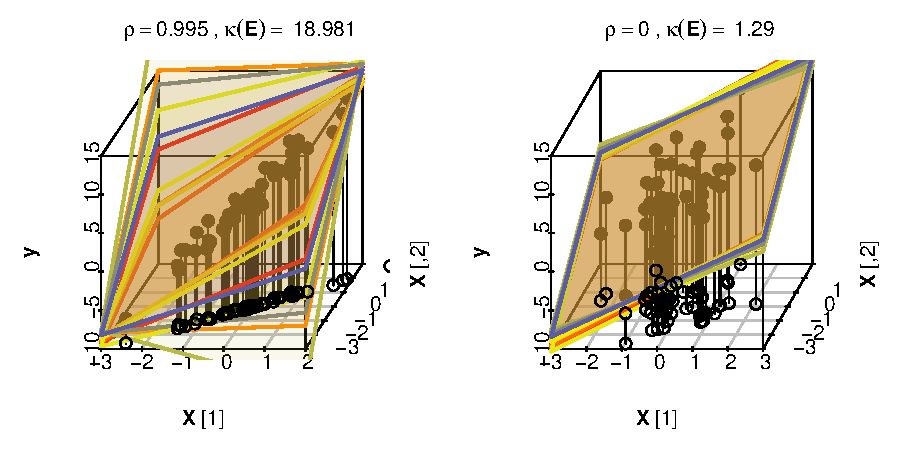
\includegraphics[width=\maxwidth]{figure/ch02_figcond-1} 
\end{knitrout}
\vspace{-7mm}
\caption{Impact of collinearity on the instability of estimates. }\label{fig:cond_ill}
\end{figure}
%\vspace{-5mm}
This allows to tune the amount of collinearity within the system by specifying $\rho$. On the left plot it is chosen to be high with $\rho=0.995$ and on the right side low with $\rho=0$. By bootstrapping the original sample 10 times and subsequent model fitting we can visualize the instability that collinearity causes. Because when we plot the planes that represent the area where the models would see $\hy=\hat{\alpha}+\hbbeta[1]\X[,1]+\hbbeta[2]\X[,2]$ we note on the left side with high collinearity ($\kappa\left(\boldsymbol{E}\right)=18.981$) that the planes are quite different from each other, whereas on the right side ($\kappa\left(\boldsymbol{E}\right)=1.29$) they seem to be very similar and thus stable. Table~\ref{tab:vdm1} shows the corresponding variance decomposition proportion matrices $\bPi$ and the least-squares model results of the original data sets.
\begin{table}[H]
\caption{Variance decomposition matrices as introduced by Belsley in the first row and summary output of the multiple linear regression models on the second row. Left side corresponds to the example with higher collinearity and the right table for the lower.}\label{tab:vdm1}
\begin{subtable}[h]{0.45\textwidth}
\centering
% latex table generated in R 4.2.2 by xtable 1.8-4 package
% Tue Mar 21 15:31:23 2023
\begingroup\footnotesize
\begin{tabular}{rrrrr}
  \toprule
mu & cond\_ind & const & \textbf{\textit{X}}[,1] & \textbf{\textit{X}}[,2] \\ 
  \midrule
1.412 & 1.000 & 0.000 & 0.003 & 0.003 \\ 
  1.000 & 1.412 & 0.939 & 0.000 & 0.000 \\ 
  0.074 & 18.981 & 0.061 & 0.997 & 0.997 \\ 
   \bottomrule
\end{tabular}
\endgroup

\end{subtable}
\begin{subtable}[h]{0.45\textwidth}
\centering
% latex table generated in R 4.2.2 by xtable 1.8-4 package
% Tue Mar 21 15:31:23 2023
\begingroup\footnotesize
\begin{tabular}{rrrrr}
  \toprule
mu & cond\_ind & const & \textbf{\textit{X}}[,1] & \textbf{\textit{X}}[,2] \\ 
  \midrule
1.144 & 1.000 & 0.294 & 0.230 & 0.206 \\ 
  0.951 & 1.202 & 0.003 & 0.448 & 0.613 \\ 
  0.887 & 1.290 & 0.703 & 0.323 & 0.181 \\ 
   \bottomrule
\end{tabular}
\endgroup

\end{subtable}
%\end{table}
\centering
\begin{subtable}[h]{0.45\textwidth}
\vspace{0.2cm}
% latex table generated in R 4.2.2 by xtable 1.8-4 package
% Tue Mar 21 15:31:23 2023
\begingroup\footnotesize
\begin{tabular}{rrrrr}
  \toprule
 & $\hat\beta$ & $\text{se}\left(\hat\beta\right)$ & $t$-value & $p$-value \\ 
  \midrule
Intercept & 4.17 & 0.17 & 24.89 & $<$ 0.0001 \\ 
  x1 & 2.35 & 1.61 & 1.46 & 0.15 \\ 
  x2 & 1.85 & 1.58 & 1.17 & 0.25 \\ 
   \bottomrule
\end{tabular}
\endgroup

\end{subtable}
\centering
\begin{subtable}[h]{0.45\textwidth}
\vspace{0.2cm}
% latex table generated in R 4.2.2 by xtable 1.8-4 package
% Tue Mar 21 15:31:23 2023
\begingroup\footnotesize
\begin{tabular}{rrrrr}
  \toprule
 & $\hat\beta$ & $\text{se}\left(\hat\beta\right)$ & $t$-value & $p$-value \\ 
  \midrule
Intercept & 4.17 & 0.17 & 24.89 & $<$ 0.0001 \\ 
  x1 & 2.16 & 0.18 & 12.19 & $<$ 0.0001 \\ 
  x2 & 2.13 & 0.15 & 14.08 & $<$ 0.0001 \\ 
   \bottomrule
\end{tabular}
\endgroup

\end{subtable}
\end{table}


But why going trough all the trouble with collinear variables and the detrimental effects that come with it and not simply drop one or some of the affected variables? Figure~\ref{fig:coll2} visualizes the model fits when the variable $\X[,2]$ is neglected although truly it has very well an effect on $\y$ as is visible in Equation~\eqref{eq:simplemodel}. We see on the right plot for low collinearity the 95\% confidence interval for $\hbbeta[1]$ does cover the true effect of 2 whereas for the case with high collinearity this seems to be not the case.
This demonstrates that it is not so easy to simply get rid of some variables as this may introduce bias to some extent.

\begin{figure}[h]%H is strict!
\centering
\begin{knitrout}
\definecolor{shadecolor}{rgb}{0.969, 0.969, 0.969}\color{fgcolor}
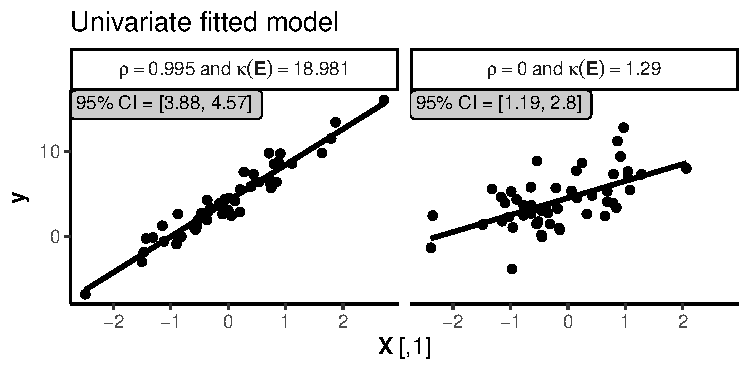
\includegraphics[width=\maxwidth]{figure/ch02_figcoll2-1} 
\end{knitrout}
\vspace{-5mm}
\caption{Univariate fitted model (\texttt{y$\sim$x1}) of the same data sets as in Figure~\ref{fig:cond_ill}. The slope of the line represents $\hbbeta[1]$ which would be truly 2 and the confidence interval thereof is given in the box. Obviously, only the right plot with low collinearity seems to capture the true effect whereas with higher collinearity the estimate is biased.}\label{fig:coll2}
\end{figure}


%%%%%%%%%%%%%%%%%%%%%%%%%%%%%%%%%%%%%%%%%%%%%%%%%%%%%%%%%%%%%%%%%%%%%%%%%%%%%%%%
%\newpage
\section{Differences between \texttt{lm} and \texttt{tram::Lm}}
%%%%%%%%%%%%%%%%%%%%%%%%%%%%%%%%%%%%%%%%%%%%%%%%%%%%%%%%%%%%%%%%%%%%%%%%%%%%%%%%

The parametrization and the chosen estimation approaches differ between \texttt{lm} and 
\texttt{tram::Lm} and in this section we are going to compare what these differences mean from a theoretical perspective.

% %%%%%%%%%%%%
\subsection{Maximum-Likelihood estimation for the linear regression model}\label{sec:mlnlm}
% %%%%%%%%%%%%

We can show that independent of the estimating procedure, with the parametrization as specified in Equation \eqref{eq:lspara} we will end up at the very same optimization problem if we go over the profile likelihood.
The approximate log-likelihood of a sample that is treated as exact is
\begin{align}
\ell(\boldsymbol{\beta},\sigma|\y)&=-N\log\left(\sigma\right)-\frac{N}{2}\log\left(2\pi\right)-\frac{1}{2}\sum_{i=1}^N\left(-\frac{\alpha}{\sigma}+\frac{1}{\sigma} \y[i]-\boldsymbol{\tilde{X}}[i,]\frac{\boldsymbol{\tilde\beta}}{\sigma}\right)^2 \nonumber\\
&=-N\log\left(\sigma\right)-\frac{N}{2}\log\left(2\pi\right)-\frac{1}{2\sigma^2}\sum_{i=1}^N\left(\y[i]-\alpha-\boldsymbol{\tilde{X}}[i,]\boldsymbol{\tilde\beta}\right)^2 \nonumber\\
&=-N\log\left(\sigma\right)-\frac{N}{2}\log\left(2\pi\right)-\frac{1}{2\sigma^2}\left(\y-\X\bbeta\right)^\top\left(\y-\X\bbeta\right) \label{eq:ll_ls}
\end{align}
We can now employ the profile likelihood where we treat $\sigma$ as the nuisance parameter:
\begin{align*}
\frac{d\ell(\boldsymbol{\beta},\sigma|\y)}{d\sigma}\Big|_{\hat\sigma}=-N\sigma^{-1}+\hat\sigma^{-3}\left(\boldsymbol{y}-\boldsymbol{X\beta}\right)^\top\left(\boldsymbol{y}-\boldsymbol{X\beta}\right)&\stackrel{!}{=}0 \\
\hat\sigma^{-3}\left(\boldsymbol{y}-\boldsymbol{X\beta}\right)^\top\left(\boldsymbol{y}-\boldsymbol{X\beta}\right)&\stackrel{!}{=}N\hat\sigma^{-1}\\
\hat\sigma^2&\stackrel{!}{=}\left(\boldsymbol{y}-\boldsymbol{X\beta}\right)^\top\left(\boldsymbol{y}-\boldsymbol{X\beta}\right)/N
\end{align*}
Plugging $\hat\sigma$ into \eqref{eq:ll_ls}, we see that $\hat\sigma$ vanishes from the equation which is handy:
\begin{align*}
\frac{d\ell(\boldsymbol{\beta},\hat\sigma|\y)}{d\boldsymbol{\beta}}\Big|_{\hbbeta}=-N\log\left(\left(\boldsymbol{y}-\boldsymbol{X\beta}\right)^\top\left(\boldsymbol{y}-\boldsymbol{X\beta}\right)\right)\frac{d}{d\boldsymbol{\beta}}\Big|_{\hbbeta}&\stackrel{!}{=}0\\
\log\left(\left(\boldsymbol{y}-\boldsymbol{X\beta}\right)^\top\left(\boldsymbol{y}-\boldsymbol{X\beta}\right)\right)\frac{d}{d\boldsymbol{\beta}}\Big|_{\hbbeta}&\stackrel{!}{=}0
\end{align*}
Since the log is a monotone function, the maximum likelihood is also found by minimizing the term $\left(\boldsymbol{y}-\boldsymbol{X\beta}\right)^\top\left(\boldsymbol{y}-\boldsymbol{X\beta}\right)$ with respect to $\boldsymbol{\beta}$ and thus the maximum-likelihood estimator $\boldsymbol{\hat\beta}$ is the very same as for the least-squares estimator described in


% %%%%%%%%%%%%
\subsection{Maximum-Likelihood estimation for the transformation model equivalent (\texttt{tram::Lm})}\label{sec:mltramLM}
% %%%%%%%%%%%%

The approximate log-likelihood with the parametrization used for the \texttt{tram::Lm} model specified in Equation~\eqref{eq:ll_trans} is
\begin{align}
\ell(\bbeta_\text{tram},\theta_0,\theta_1|\y)&=+N\log(\theta_1)-\frac{N}{2}\log\left(2\pi\right)-\frac{1}{2}\sum_{i=1}^N\left(\theta_0+\theta_1 \y[i]-\boldsymbol{\tilde{X}}[i,]\bbeta_\text{tram}\right)^2
\label{eq:ll_tramLm}
\end{align}
which has one parameter ($\theta_1$) more to simultaneously estimate.

The design matrix in this setup is different. For \texttt{lm}, $\X$ contained the variables that will be used to explain the outcome $\y$. But this can also be reformulated in terms of using the \textit{variables including the outcome} to explain the  \textit{error} $\bvarepsilon[i]\sim \N(0,1)$.
Since for \texttt{tram::Lm} the parameter $\theta_1$ is attached to the outcome $\y$, the collinearity constellation is not only restricted to the $\X$ space but extends onto $\left[\y,\X\right]$.
This basically implies that the better the outcome $\y$ is explainable by $\X$, the higher the collinearity and thus the larger the effects caused by it. This is important to keep in mind.

\begin{figure}[h]%H is strict!
\begin{center}
\begin{knitrout}
\definecolor{shadecolor}{rgb}{0.969, 0.969, 0.969}\color{fgcolor}
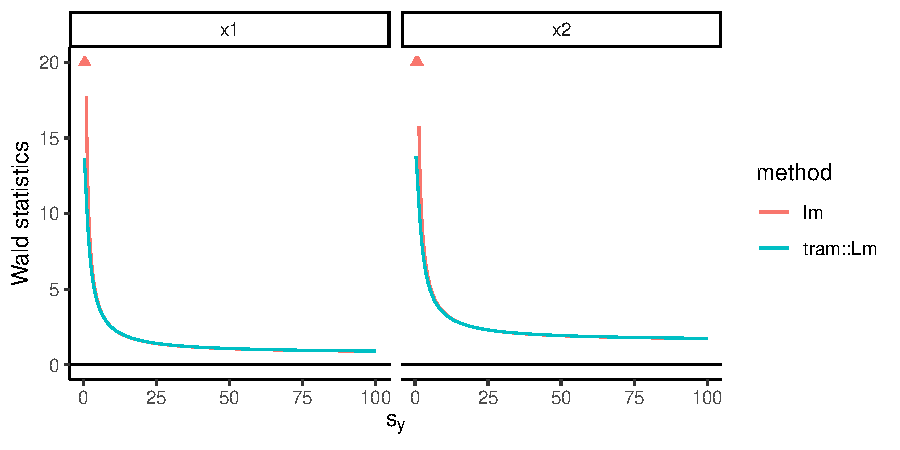
\includegraphics[width=\maxwidth]{figure/ch02_figcolllikelihood-1} 
\end{knitrout}
\end{center}
\caption{Simulating data as $\y=10+2\x_1+2\x_2+s_y\cdot \bvarepsilon$ with $\left(\x_1,\x_2,\bvarepsilon\right)\sim\N_{3n}(0,1),n=100$. The scaling factor $s_y$ is iterated on a grid between 0.3333333 and 100 where a low scaling factor means that the outcome $\y$ is well explainable and thus collinearity for \texttt{tram::Lm} is higher. Wald statistics are plotted restricted to have maximum values of 20 and points laying above are illustrated as triangles.}
\label{fig:colllikelihood}
\end{figure}









%%%%%%%%%%%%%%%%%%%%%%%%%%%%%%%%%%%%%%%%%%%%%%%%%%%%%%%%%%%%%%%%%%%%%%

\appendix

% LaTeX file for Chapter 01


%%%%%%%%%%%%%%%%%%%%%%%%%%%%%%%%%%%%%%%%%%%%%%%%%%%%%%%%%%%%%%%%%%%%%%%%%%%%%%%%
\chapter{Appendix}
%%%%%%%%%%%%%%%%%%%%%%%%%%%%%%%%%%%%%%%%%%%%%%%%%%%%%%%%%%%%%%%%%%%%%%%%%%%%%%%%



%%%%%%%%%%%%%%%%%%%%%%%%%%%%%%%%%%%%%%%%%%%%%%%%%%%%%%%%%%%%%%%%%%%%%%%%%%%%%%%%
\section{Approximate likelihood}\label{sec:approxlikelihood}
%%%%%%%%%%%%%%%%%%%%%%%%%%%%%%%%%%%%%%%%%%%%%%%%%%%%%%%%%%%%%%%%%%%%%%%%%%%%%%%%
Since real-life data is always observed in intervals $\boldsymbol{D}=(\underline{y},\overline{y}]$ and is never exact (although treated as if), the likelihood contribution of one observation is:
\begin{align*}
l(\boldsymbol{\beta_\tram,\theta}|\boldsymbol{D})=\bfP(\underline{y}< Y\leq \overline{y}|\boldsymbol{X}=\boldsymbol{x})=F_Z\left(h_Y(\overline{y}|\boldsymbol{\theta})-\boldsymbol{\tilde{x}}\boldsymbol{\beta_\tram}\right)-F_Z\left(h_Y(\underline{y}|\boldsymbol{\theta})-\boldsymbol{\tilde{x}}\boldsymbol{\beta_\tram}\right)
\end{align*}
which is the exact likelihood as originally introduced by Fisher. The approximated likelihood for a continuous response is obtained by making the interval around the "observed" value $y$ negligibly small $\boldsymbol{D}=(y-\epsilon,y+\epsilon]$ and thus the likelihood is approximated as
\begin{align*}
l(\boldsymbol{\beta_\tram,\theta}|\boldsymbol{D})&=F_Z\left(h_Y(y+\epsilon|\boldsymbol{\theta})-\boldsymbol{\tilde{x}}\boldsymbol{\beta_\tram}\right)-F_Z\left(h_Y(y-\epsilon|\boldsymbol{\theta})-\boldsymbol{\tilde{x}}\boldsymbol{\beta_\tram}\right)\\
&=\int_{y-\epsilon}^{y+\epsilon}F_Z'\left(h_Y(u|\boldsymbol{\theta})-\boldsymbol{\tilde{x}}\boldsymbol{\beta_\tram}\right)h_Y'(u|\boldsymbol{\theta})du\\
&\approx f_Z\left(h_Y(y|\boldsymbol{\theta})-\boldsymbol{\tilde{x}}\boldsymbol{\beta_\tram}\right)h_Y'(y|\boldsymbol{\theta})\cdot 2\epsilon\\
&\propto f_Z\left(h_Y(y|\boldsymbol{\theta})-\boldsymbol{\tilde{x}}\boldsymbol{\beta_\tram}\right)h_Y'(y|\boldsymbol{\theta})
\end{align*}
The joint likelihood for several observations assuming independence is:
\begin{align*}
L(\boldsymbol{\beta_\tram,\theta}|\boldsymbol{D_1,...,D_N})=\prod_{i=1}^N l(\boldsymbol{\beta_\tram,\theta}|\boldsymbol{D_i})
\end{align*}
where it is theoretically and computationally convenient to operate on the log scale
\begin{align*}
\ell(\boldsymbol{\beta_\tram,\theta}|\boldsymbol{D_1,...,D_N})=\sum_{i=1}^N \log\left(l(\boldsymbol{\beta_\tram,\theta}|\boldsymbol{D_i})\right)
\end{align*}
The resulting maximum log-likelihood estimator is then:
\begin{align*}
\boldsymbol{\hat{\beta}_\tram,\hat\theta}=\argmax \ell(\boldsymbol{\beta_\tram,\theta}|\boldsymbol{D_1,...,D_N})
\end{align*}


%%%%%%%%%%%%%%%%%%%%%%%%%%%%%%%%%%%%%%%%%%%%%%%%%%%%%%%%%%%%%%%%%%%%%%%%%%%%%%%%
\newpage
\section{Computational reproducibility}\label{sec:repro}
%%%%%%%%%%%%%%%%%%%%%%%%%%%%%%%%%%%%%%%%%%%%%%%%%%%%%%%%%%%%%%%%%%%%%%%%%%%%%%%%




\newpage
\begin{knitrout}
\definecolor{shadecolor}{rgb}{0.969, 0.969, 0.969}\color{fgcolor}\begin{kframe}
\begin{alltt}
\hlkwd{sessionInfo}\hlstd{()}
\end{alltt}
\begin{verbatim}
## R version 4.2.2 Patched (2022-11-10 r83330)
## Platform: x86_64-pc-linux-gnu (64-bit)
## Running under: Ubuntu 20.04.5 LTS
## 
## Matrix products: default
## BLAS:   /usr/lib/x86_64-linux-gnu/blas/libblas.so.3.9.0
## LAPACK: /usr/lib/x86_64-linux-gnu/lapack/liblapack.so.3.9.0
## 
## locale:
##  [1] LC_CTYPE=de_CH.UTF-8       LC_NUMERIC=C              
##  [3] LC_TIME=de_CH.UTF-8        LC_COLLATE=de_CH.UTF-8    
##  [5] LC_MONETARY=de_CH.UTF-8    LC_MESSAGES=de_CH.UTF-8   
##  [7] LC_PAPER=de_CH.UTF-8       LC_NAME=C                 
##  [9] LC_ADDRESS=C               LC_TELEPHONE=C            
## [11] LC_MEASUREMENT=de_CH.UTF-8 LC_IDENTIFICATION=C       
## 
## attached base packages:
## [1] stats     graphics  grDevices utils     datasets  methods   base     
## 
## other attached packages:
##  [1] tram_0.8-0           mlt_1.4-3            basefun_1.1-2       
##  [4] variables_1.1-1      forcats_0.5.1        stringr_1.4.0       
##  [7] dplyr_1.0.9          purrr_0.3.4          readr_2.1.2         
## [10] tidyr_1.2.0          tibble_3.1.7         ggplot2_3.4.0       
## [13] tidyverse_1.3.1      RColorBrewer_1.1-3   xtable_1.8-4        
## [16] biostatUZH_2.0.2     MASS_7.3-58          survival_3.4-0      
## [19] tableone_0.13.2      Collinearity_1.1.2   mvtnorm_1.1-3       
## [22] scales_1.2.0         scatterplot3d_0.3-41 knitr_1.39          
## 
## loaded via a namespace (and not attached):
##  [1] nlme_3.1-160        fs_1.5.2            cmprsk_2.2-11      
##  [4] lubridate_1.8.0     httr_1.4.3          numDeriv_2016.8-1.1
##  [7] tools_4.2.2         backports_1.4.1     utf8_1.2.2         
## [10] R6_2.5.1            mgcv_1.8-41         DBI_1.1.2          
## [13] colorspace_2.0-3    withr_2.5.0         tidyselect_1.1.2   
## [16] compiler_4.2.2      orthopolynom_1.0-6  cli_3.4.1          
## [19] rvest_1.0.2         alabama_2022.4-1    xml2_1.3.3         
## [22] sandwich_3.0-1      labeling_0.4.2      quadprog_1.5-8     
## [25] digest_0.6.29       minqa_1.2.4         pkgconfig_2.0.3    
## [28] lme4_1.1-29         dbplyr_2.1.1        highr_0.9          
## [31] rlang_1.0.6         readxl_1.4.0        rstudioapi_0.13    
## [34] farver_2.1.0        generics_0.1.2      zoo_1.8-10         
## [37] jsonlite_1.8.0      magrittr_2.0.3      polynom_1.4-1      
## [40] Formula_1.2-4       coneproj_1.16       Matrix_1.5-1       
## [43] Rcpp_1.0.8.3        munsell_0.5.0       fansi_1.0.3        
## [46] lifecycle_1.0.3     stringi_1.7.6       multcomp_1.4-19    
## [49] BB_2019.10-1        grid_4.2.2          crayon_1.5.1       
## [52] lattice_0.20-45     haven_2.5.0         splines_4.2.2      
## [55] hms_1.1.1           pillar_1.7.0        boot_1.3-28        
## [58] codetools_0.2-18    reprex_2.0.1        glue_1.6.2         
## [61] evaluate_0.15       mitools_2.4         modelr_0.1.8       
## [64] vctrs_0.5.1         nloptr_2.0.1        tzdb_0.3.0         
## [67] psy_1.2             cellranger_1.1.0    gtable_0.3.0       
## [70] assertthat_0.2.1    xfun_0.31           broom_0.8.0        
## [73] survey_4.1-1        TH.data_1.1-1       ellipsis_0.3.2
\end{verbatim}
\end{kframe}
\end{knitrout}





\cleardoublepage
\phantomsection
\addtocontents{toc}{\protect \vspace*{10mm}}
\addcontentsline{toc}{chapter}{\bfseries Bibliography}


\bibliographystyle{mywiley} 
\bibliography{biblio}

\cleardoublepage

\end{document}

